\documentclass{article}\usepackage[]{graphicx}\usepackage[]{color}
%% maxwidth is the original width if it is less than linewidth
%% otherwise use linewidth (to make sure the graphics do not exceed the margin)
\makeatletter
\def\maxwidth{ %
  \ifdim\Gin@nat@width>\linewidth
    \linewidth
  \else
    \Gin@nat@width
  \fi
}
\makeatother

\definecolor{fgcolor}{rgb}{0.345, 0.345, 0.345}
\newcommand{\hlnum}[1]{\textcolor[rgb]{0.686,0.059,0.569}{#1}}%
\newcommand{\hlstr}[1]{\textcolor[rgb]{0.192,0.494,0.8}{#1}}%
\newcommand{\hlcom}[1]{\textcolor[rgb]{0.678,0.584,0.686}{\textit{#1}}}%
\newcommand{\hlopt}[1]{\textcolor[rgb]{0,0,0}{#1}}%
\newcommand{\hlstd}[1]{\textcolor[rgb]{0.345,0.345,0.345}{#1}}%
\newcommand{\hlkwa}[1]{\textcolor[rgb]{0.161,0.373,0.58}{\textbf{#1}}}%
\newcommand{\hlkwb}[1]{\textcolor[rgb]{0.69,0.353,0.396}{#1}}%
\newcommand{\hlkwc}[1]{\textcolor[rgb]{0.333,0.667,0.333}{#1}}%
\newcommand{\hlkwd}[1]{\textcolor[rgb]{0.737,0.353,0.396}{\textbf{#1}}}%

\usepackage{framed}
\makeatletter
\newenvironment{kframe}{%
 \def\at@end@of@kframe{}%
 \ifinner\ifhmode%
  \def\at@end@of@kframe{\end{minipage}}%
  \begin{minipage}{\columnwidth}%
 \fi\fi%
 \def\FrameCommand##1{\hskip\@totalleftmargin \hskip-\fboxsep
 \colorbox{shadecolor}{##1}\hskip-\fboxsep
     % There is no \\@totalrightmargin, so:
     \hskip-\linewidth \hskip-\@totalleftmargin \hskip\columnwidth}%
 \MakeFramed {\advance\hsize-\width
   \@totalleftmargin\z@ \linewidth\hsize
   \@setminipage}}%
 {\par\unskip\endMakeFramed%
 \at@end@of@kframe}
\makeatother

\definecolor{shadecolor}{rgb}{.97, .97, .97}
\definecolor{messagecolor}{rgb}{0, 0, 0}
\definecolor{warningcolor}{rgb}{1, 0, 1}
\definecolor{errorcolor}{rgb}{1, 0, 0}
\newenvironment{knitrout}{}{} % an empty environment to be redefined in TeX

\usepackage{alltt}
\usepackage{float, hyperref}
\usepackage[margin=1in]{geometry}
\usepackage{graphicx}
\usepackage{hyperref}
\IfFileExists{upquote.sty}{\usepackage{upquote}}{}

\begin{document}

\author{Lindsay Rutter}
\title{Stat.585X: Draft of Project Plan}

\maketitle




\section*{Project Topic}

The project will focus on the construction and interactive visualization of phylogenetic representation of soybean varieties.

\section*{Project Motivation}

The motivation of the project stems from my interest in bioinformatics and computational biology. Ideally, the product could be used by biologists, geneticists, and agronomists interested in studying how soybean varieties are related. By referencing the interactive visualization of the phylogenetic tree, these scientists may better understand genetic testing results - in this particular dataset, in terms of copy number variants, single nucleotide polymorphisms, protein content, and yield - and use that knowledge in future breeding.

\section*{Available Data}

The available data consists of a data frame structure that contains 412 direct child-parent relationships between pairs of soybean varieties. These data were collected from frield trials, genetic studies, and United States Department of Agriculture (USDA) bulletins, and date as early as the first decade of the 1900s.

\section*{Data Collection and Processing}

The data frame format of the soybean varieties has been represented as an interactive phylogenetic tree, in Shiny software produced by Susan VanderPlas:\\

\hyperref[shinySBLink]{http://gsoja.agron.iastate.edu:3838/Soybeans/}\\

\noindent
In the "Genealogy" tab of the Shiny application, the user may choose one or more varieties in the left-panel menu, and immediately view the phylogenetic tree representation of the selected varieties in the right-panel plot as per reactive programming.\\

However, currently, the right-panel plots are plotted independently for each soybean variety selected, showing a user-selected number of generations surrounding that variety, regardless of its relationship to any other varieties selected.\\

Instead, it may be useful for biologists to obtain one large plot in the right-panel that merges the selected soybean varieties, thereby determining not only whether or not there exists a relationship between the varieties, but also showing the relationship as a path in the graphical phylogetntic structure, with possibly the varieties (nodes) and the path (edges) between them highlighted for emphasis.\\

In total, there are about 230 unique soybean varieties present in the tree data frame. The package igraph might be used to determine any pathway relationships between selected varities:\\

\hyperref[igraphLink]{http://cran.r-project.org/web/packages/igraph/index.html}\\

\noindent

\section*{Final Product}

If the Shiny application is properly functioning, it will then be extensively commented in the format that will soon be taught in class. This may bring the application one step closer to being available to interested users via an R Package.

\section*{Progress as of April 9}

1. The first step was examining the data, and perform data cleaning to ensure there are no obvious errors or counterintuitive information about the soybean varieties.

\begin{itemize}

\item I discovered that there are many soybean nodes that do not have a year ({\tt NA}). I plan to simply taking the average of all relationships and using that for these cases (which seems to be ~9 years). 

\begin{knitrout}
\definecolor{shadecolor}{rgb}{0.969, 0.969, 0.969}\color{fgcolor}\begin{kframe}
\begin{alltt}
\hlkwd{setwd}\hlstd{(}\hlstr{"/Users/MacOwner/Desktop/Cook/SBTree"}\hlstd{)}

\hlcom{####################### NECESSARY PACKAGES AND RESOURCES #######################}
\hlkwd{library}\hlstd{(plyr)}
\hlkwd{load}\hlstd{(}\hlstr{"tree.rda"}\hlstd{)}

\hlcom{###################### TEST GENERATIONAL AGE DIFF #############################}

\hlcom{# This produces year_rltnshp, which is a data.frame with 412 rows from the}
\hlcom{# original tree file However, there are 5 columns that list (in order) child}
\hlcom{# name, parent name, year of child, year of parent, and the difference}
\hlcom{# between the year of child minus year of parent (which should be positive)}

\hlstd{year_rltnshp} \hlkwb{<-} \hlkwd{data.frame}\hlstd{(}\hlkwc{child} \hlstd{=} \hlkwd{character}\hlstd{(),} \hlkwc{par} \hlstd{=} \hlkwd{character}\hlstd{(),} \hlkwc{child_yr} \hlstd{=} \hlkwd{integer}\hlstd{(}\hlnum{0}\hlstd{),}
    \hlkwc{par_yr} \hlstd{=} \hlkwd{integer}\hlstd{(}\hlnum{0}\hlstd{),} \hlkwc{diff} \hlstd{=} \hlkwd{integer}\hlstd{(}\hlnum{0}\hlstd{),} \hlkwc{stringsAsFactors} \hlstd{=} \hlnum{FALSE}\hlstd{)}

\hlkwa{for} \hlstd{(i} \hlkwa{in} \hlnum{1}\hlopt{:}\hlkwd{dim}\hlstd{(tree)[}\hlnum{1}\hlstd{]) \{}
    \hlstd{child} \hlkwb{=} \hlstd{tree}\hlopt{$}\hlstd{child[i]}
    \hlstd{par} \hlkwb{=} \hlstd{tree}\hlopt{$}\hlstd{parent[i]}
    \hlstd{child_yr} \hlkwb{=} \hlstd{tree}\hlopt{$}\hlstd{year[i]}
    \hlstd{par_yr} \hlkwb{=} \hlkwd{subset}\hlstd{(tree, tree}\hlopt{$}\hlstd{child} \hlopt{==} \hlstd{par)}\hlopt{$}\hlstd{year[}\hlnum{1}\hlstd{]}
    \hlstd{age_diff} \hlkwb{=} \hlstd{child_yr} \hlopt{-} \hlstd{par_yr}
    \hlstd{new_row} \hlkwb{=} \hlkwd{c}\hlstd{(child, par, child_yr, par_yr, age_diff)}
    \hlstd{year_rltnshp[i, ]} \hlkwb{=} \hlstd{new_row}
\hlstd{\}}

\hlcom{# This produces year_rltnshp_noNA, which is a subset of year_rltnshp, except}
\hlcom{# that it only contains the 301 rows where there is a calculated value for}
\hlcom{# the column representing the difference between child year minus parent}
\hlcom{# year}

\hlstd{year_rltnship_noNA} \hlkwb{=} \hlkwd{subset}\hlstd{(year_rltnshp, year_rltnshp}\hlopt{$}\hlstd{diff} \hlopt{!=} \hlstr{"NA"}\hlstd{)}

\hlcom{# I did summary of the generation difference for the 301 cases where its}
\hlcom{# value could be calculated. Oddly, the minimum value was negative, (I}
\hlcom{# think) meaning that the child is older than the parent!}

\hlkwd{min}\hlstd{(}\hlkwd{as.numeric}\hlstd{(year_rltnship_noNA}\hlopt{$}\hlstd{diff))}  \hlcom{#-16.5}
\end{alltt}
\begin{verbatim}
## [1] -16.5
\end{verbatim}
\begin{alltt}
\hlkwd{max}\hlstd{(}\hlkwd{as.numeric}\hlstd{(year_rltnship_noNA}\hlopt{$}\hlstd{diff))}  \hlcom{#54}
\end{alltt}
\begin{verbatim}
## [1] 54
\end{verbatim}
\begin{alltt}
\hlkwd{mean}\hlstd{(}\hlkwd{as.numeric}\hlstd{(year_rltnship_noNA}\hlopt{$}\hlstd{diff))}  \hlcom{#9.174419}
\end{alltt}
\begin{verbatim}
## [1] 9.174
\end{verbatim}
\end{kframe}
\end{knitrout}


\item Another problem I found when cleaning the data, is that there are 16 cases where the parent {\tt year} is younger than (or equal to) the child {\tt year}. For these cases, I also looked at the variable {\tt min.repro.year} in {\tt tree.rda}, but that did not solve the problem. 

\begin{knitrout}
\definecolor{shadecolor}{rgb}{0.969, 0.969, 0.969}\color{fgcolor}\begin{kframe}
\begin{alltt}
\hlcom{# I created negRltnshp, a subset of the year_rltnship_noNA where the}
\hlcom{# generational difference was less than or equal to zero. This resulted in}
\hlcom{# 16 pairs. I also looked at these pairs and tried to determine if using the}
\hlcom{# min.repro.year instead from the original tree would fix these problems,}
\hlcom{# but it did not always.}

\hlstd{negRltshp} \hlkwb{=} \hlkwd{subset}\hlstd{(year_rltnship_noNA, year_rltnship_noNA}\hlopt{$}\hlstd{diff} \hlopt{<=} \hlnum{0}\hlstd{)}
\end{alltt}
\end{kframe}
\end{knitrout}


\item What I did to discover this issue is in {\tt testTree.R}. The 16 cases are stored in the variable {\tt negRltshp}.

\begin{knitrout}
\definecolor{shadecolor}{rgb}{0.969, 0.969, 0.969}\color{fgcolor}\begin{kframe}
\begin{alltt}
\hlstd{negRltshp}
\end{alltt}
\begin{verbatim}
##                  child        par child_yr par_yr  diff
## 17             Bradley     J74-39     1975   1975     0
## 48            D55-4090      Ogden     1945   1953    -8
## 64                Dare    D52-810     1962   1964    -2
## 66      Davis x Peking      Davis     1958   1966    -8
## 87              Hagood Centennial     1977   1977     0
## 108                L15      Wayne     1960   1966    -6
## 139            N45-745      Ogden   1951.5   1953  -1.5
## 155        Ogden x CNS      Ogden     1945   1953    -8
## 178             Ransom   D56-1185     1958   1963    -5
## 200              Wells      C1253     1947   1961   -14
## 251           D49-2510      S 100     1945   1945     0
## 274             Dillon Centennial     1977   1977     0
## 282              Essex   S55-7075     1962   1963    -1
## 386 Renville x Capital   Renville     1964   1964     0
## 396             T80-69     J74-40     1975   1975     0
## 406              Wells     C1266R     1947 1963.5 -16.5
\end{verbatim}
\end{kframe}
\end{knitrout}


\end{itemize}

2. I spoke with scientists and computiational scientists who know more about why these problems may exist in the data. 

\begin{itemize}

\item Susan VanderPlas explained that the year introduced and year registered can be different by up to 30 years for a given variety, and that this can explain the many cases of children being older than their parents
  
\item It was suggested to me to throw a flag (message) to the user if a child is older than the parent, and indicate to them that the years were forced (imputated) such that the variety is younger than its parents and older than its children

\end{itemize}

3. Along with Susan and Dr. Cook, I observed the available Shiny applet:\\

\hyperref[shinySBLink]{http://gsoja.agron.iastate.edu:3838/Soybeans/}\\

and thought that the greatest-grandparents of the varieties seemed to be {\tt Tokyo} and {\tt AK\_004}. As such, I wanted to determine whether or not these two varieties could encompass the majority of the rest of the varieties.\\

So, I added code to the script  {\tt testTree.R} and the relevant lines for me to determine lines that may not be in the union between these two potentially greatest-grandparent varieties:\\

\begin{knitrout}
\definecolor{shadecolor}{rgb}{0.969, 0.969, 0.969}\color{fgcolor}\begin{kframe}
\begin{alltt}
\hlkwd{setwd}\hlstd{(}\hlstr{"/Users/MacOwner/Desktop/Cook/SBTree"}\hlstd{)}

\hlcom{####################### NECESSARY PACKAGES AND RESOURCES #######################}
\hlkwd{library}\hlstd{(plyr)}
\hlkwd{load}\hlstd{(}\hlstr{"tree.rda"}\hlstd{)}

\hlcom{################## TEST TOTAL NODES IN ALL-ENCOMPASSING TREE ###########################}

\hlcom{# There are 206 unique 'child' in the 'tree'}
\hlstd{uniqueChild} \hlkwb{=} \hlkwd{sort}\hlstd{(}\hlkwd{unique}\hlstd{(tree}\hlopt{$}\hlstd{child))}
\hlcom{# There are 165 unique 'parent' in the 'tree'}
\hlstd{uniqueParent} \hlkwb{=} \hlkwd{sort}\hlstd{(}\hlkwd{unique}\hlstd{(tree}\hlopt{$}\hlstd{parent))}
\hlcom{# There are 230 unique nodes in the 'tree'}
\hlstd{uniqueNode} \hlkwb{=} \hlkwd{sort}\hlstd{(}\hlkwd{union}\hlstd{(uniqueChild, uniqueParent))}

\hlcom{# These lines were used to generate the nodes from the two large trees}
\hlcom{# (Tokyo and AK_004).  The resulting variables were saved to the working}
\hlcom{# directory tokyoNodes = vals$df AK004Nodes = vals$df save(tokyoNodes,}
\hlcom{# file='tokyoNodes') save(AK004Nodes, file='AK004Nodes')}

\hlkwd{load}\hlstd{(}\hlstr{"tokyoNodes"}\hlstd{)}
\hlkwd{load}\hlstd{(}\hlstr{"AK004Nodes"}\hlstd{)}

\hlcom{# There are 91 unique child in 'Tokyo'}
\hlstd{uniqueTokyoChild} \hlkwb{=} \hlkwd{unique}\hlstd{(tokyoNodes}\hlopt{$}\hlstd{label)}
\hlcom{# There are 61 unique parents in 'Tokyo'}
\hlstd{uniqueTokyoParent} \hlkwb{=} \hlkwd{unique}\hlstd{(tokyoNodes}\hlopt{$}\hlstd{root)}
\hlcom{# There are 91 unique nodes in 'Tokyo'}
\hlstd{uniqueTokyoNode} \hlkwb{=} \hlkwd{union}\hlstd{(uniqueTokyoChild, uniqueTokyoParent)}

\hlcom{# There are 104 unique child in 'AK_004'}
\hlstd{uniqueAK004Child} \hlkwb{=} \hlkwd{unique}\hlstd{(AK004Nodes}\hlopt{$}\hlstd{label)}
\hlcom{# There are 67 unique child in 'AK_004'}
\hlstd{uniqueAK004Parent} \hlkwb{=} \hlkwd{unique}\hlstd{(AK004Nodes}\hlopt{$}\hlstd{root)}
\hlcom{# There are 104 unique nodes in 'AK_004'}
\hlstd{uniqueAK004Node} \hlkwb{=} \hlkwd{union}\hlstd{(uniqueAK004Child, uniqueAK004Parent)}

\hlcom{# There are 143 unique nodes in 'AK_004' and 'Tokyo'}
\hlstd{tokyoAK004Union} \hlkwb{=} \hlkwd{sort}\hlstd{(}\hlkwd{union}\hlstd{(uniqueTokyoNode, uniqueAK004Node))}

\hlcom{# There are 52 nodes in the intersection}
\hlstd{tokyoAK004Int} \hlkwb{=} \hlkwd{intersect}\hlstd{(uniqueTokyoNode, uniqueAK004Node)}

\hlcom{# There are 87 nodes not in Tokyo and AK_004 (230-143)}
\hlstd{notInTokyoAK004} \hlkwb{=} \hlstd{uniqueNode[}\hlopt{!}\hlstd{(uniqueNode} \hlopt \hlstd{tokyoAK004Union)]}
\end{alltt}
\end{kframe}
\end{knitrout}


This revealed that 87 varieties are not descendants of {\tt Tokyo} and {\tt AK\_004}. So, I needed to devise a new plan to generate a complete layout of the tree.

\begin{knitrout}
\definecolor{shadecolor}{rgb}{0.969, 0.969, 0.969}\color{fgcolor}\begin{kframe}
\begin{alltt}
\hlkwd{str}\hlstd{(notInTokyoAK004)}
\end{alltt}
\begin{verbatim}
##  chr [1:87] "(Lincoln x Richland) x Korean" "Altona" "Amsoy-71" ...
\end{verbatim}
\end{kframe}
\end{knitrout}


4. I addressed this issue by creating a script called {\tt testIGraph.R}:

\begin{itemize}

\item I wanted to develop a visualization of the complete tree, as this is currently not possible in the Shiny application. As such, I created an output .csv file in this scipt that can then be read into the software {\tt Cytoscape}. The software allows for the visualization of the graph and calculation of graph theoretical parameters:\\

\hyperref[cytoscape]{http://www.cytoscape.org/}\\

\noindent using the following code:\\

\begin{knitrout}
\definecolor{shadecolor}{rgb}{0.969, 0.969, 0.969}\color{fgcolor}\begin{kframe}
\begin{alltt}
\hlcom{# Must use igraph version 0.7.0}

\hlkwd{setwd}\hlstd{(}\hlstr{"/Users/MacOwner/Desktop/Cook/SBTree"}\hlstd{)}

\hlkwd{library}\hlstd{(plyr)}
\hlkwd{library}\hlstd{(reshape2)}
\hlkwd{library}\hlstd{(ggplot2)}
\hlkwd{library}\hlstd{(stringr)}
\hlkwd{library}\hlstd{(igraph)}

\hlkwd{load}\hlstd{(}\hlstr{"tree.rda"}\hlstd{)}
\hlcom{# Total tree nodes (412*2)}
\hlstd{treeGraph} \hlkwb{=} \hlkwd{as.data.frame}\hlstd{(}\hlkwd{cbind}\hlstd{(tree}\hlopt{$}\hlstd{child, tree}\hlopt{$}\hlstd{parent))}
\hlcom{# Remove any rows with 'NA' relationship (340*2)}
\hlstd{treeGraph} \hlkwb{=} \hlstd{treeGraph[}\hlopt{-}\hlkwd{which}\hlstd{(}\hlkwd{is.na}\hlstd{(tree}\hlopt{$}\hlstd{parent)), ]}
\hlcom{# Add an edge weight to each pair of vertices (all of weight value equal to}
\hlcom{# one)}
\hlstd{treeGraph} \hlkwb{=} \hlkwd{cbind}\hlstd{(treeGraph,} \hlkwd{rep}\hlstd{(}\hlnum{1}\hlstd{,} \hlkwd{dim}\hlstd{(treeGraph)[}\hlnum{1}\hlstd{]))}
\hlcom{# Add column names the tree}
\hlkwd{colnames}\hlstd{(treeGraph)} \hlkwb{=} \hlkwd{c}\hlstd{(}\hlstr{"child"}\hlstd{,} \hlstr{"parent"}\hlstd{,} \hlstr{"edgeWt"}\hlstd{)}

\hlcom{# Write the tree as a .cvs file to be read into Cytoscape}
\hlstd{sbTreeGraph} \hlkwb{=} \hlkwd{write.csv}\hlstd{(treeGraph,} \hlstr{"sbTreeGraphTest.csv"}\hlstd{)}
\end{alltt}
\end{kframe}
\end{knitrout}


\begin{figure}[ht!]
\centering
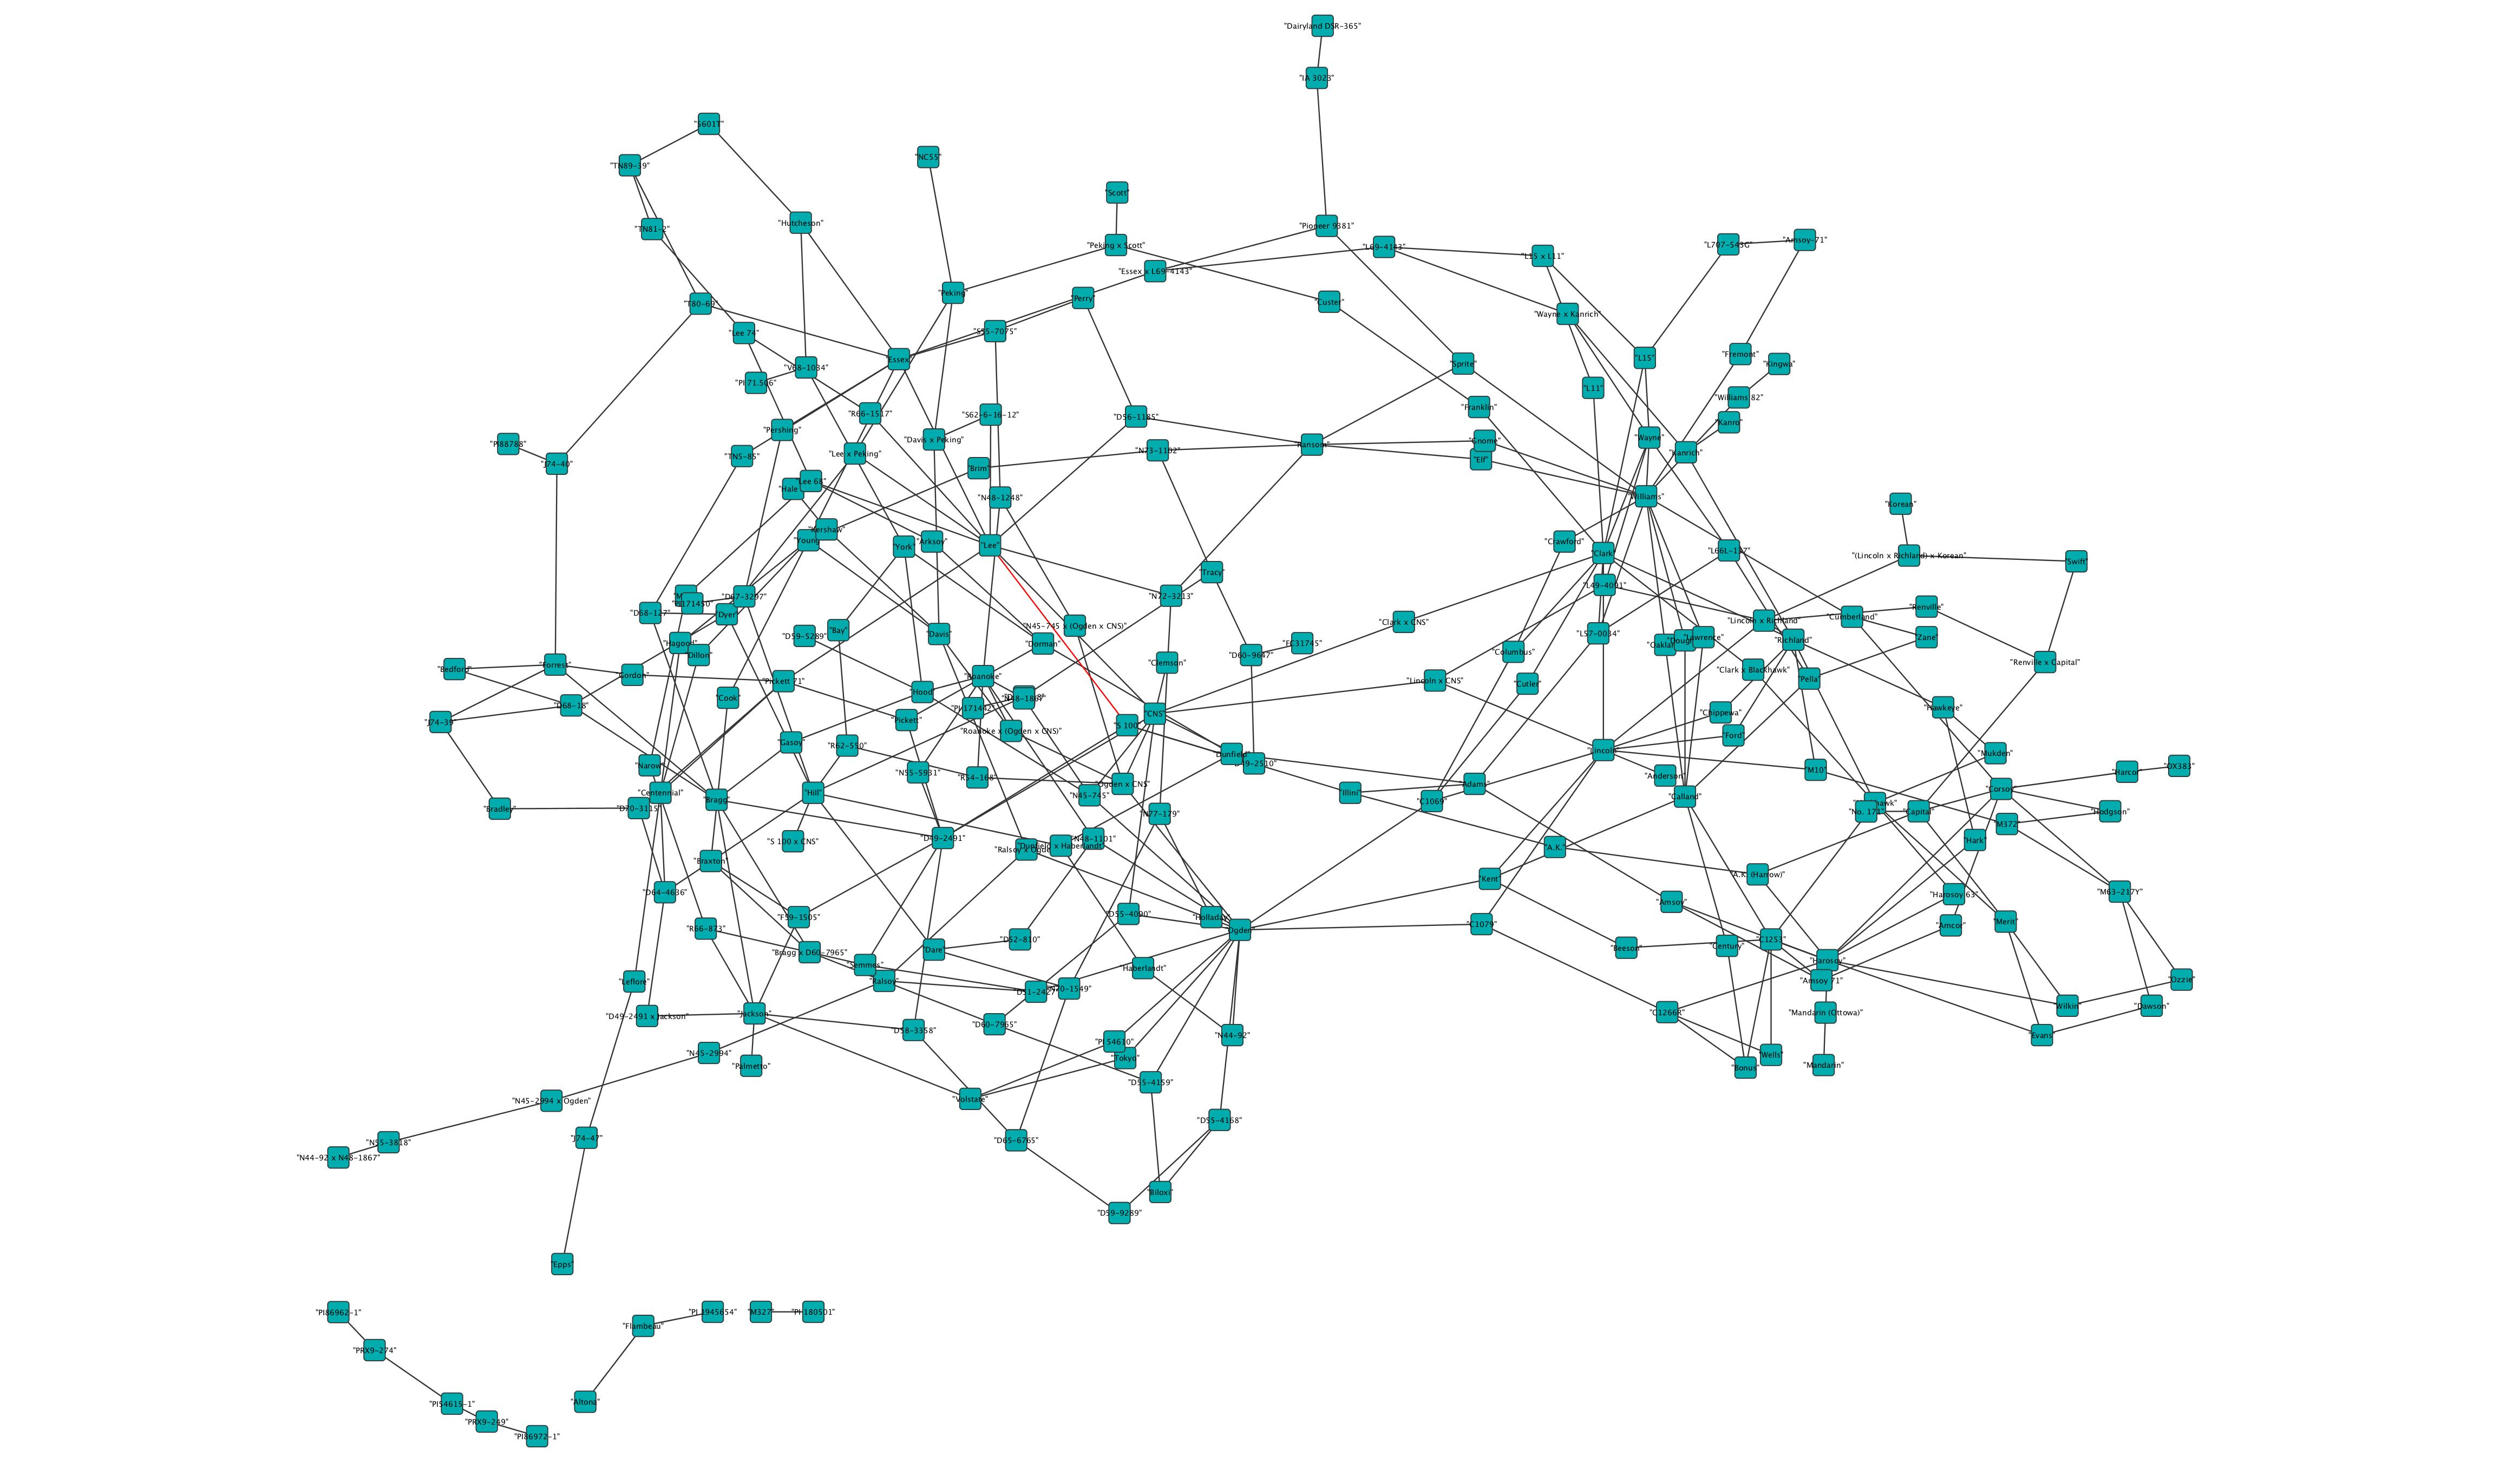
\includegraphics[width=200mm]{cytoscapeTree.jpg}
\caption{Complete Cytoscape Tree}
\label{overflow}
\end{figure}

\item I created two main functions in the {\tt testIGraph.R} script:
  \begin{itemize}
  \item getBasicStatistics()
  \item getPath()
  \end{itemize}

\item In order to run these functions that contain functions from the igraph package, I needed to convert the tree object into a graph that can be read by igraph.

\begin{knitrout}
\definecolor{shadecolor}{rgb}{0.969, 0.969, 0.969}\color{fgcolor}\begin{kframe}
\begin{alltt}
\hlcom{# Convert the data frame object into an object that can be read by igraph}
\hlcom{# package}
\hlstd{mygraph} \hlkwb{=} \hlkwd{graph.data.frame}\hlstd{(treeGraph,} \hlkwc{directed} \hlstd{= T)}
\end{alltt}
\end{kframe}
\end{knitrout}


\item I also created five test cases, knowing that lineage {\tt Falmbeau} is not connected to any other varieties, and that {\tt Brim} and {\tt Bedford} are connected by a direct ancestor/descendant path, and hence their order mattered for this directed graph. Finally, {\tt Tokyo} and {\tt Narow} could provide an example of cousins, that is not a direct ancestor/descenant lineage.

\begin{knitrout}
\definecolor{shadecolor}{rgb}{0.969, 0.969, 0.969}\color{fgcolor}\begin{kframe}
\begin{alltt}
\hlstd{v1} \hlkwb{=} \hlstr{"Brim"}
\hlstd{v2} \hlkwb{=} \hlstr{"Bedford"}
\hlstd{v3} \hlkwb{=} \hlstr{"Flambeau"}
\hlstd{v4} \hlkwb{=} \hlstr{"Tokyo"}
\hlstd{v5} \hlkwb{=} \hlstr{"Narow"}
\end{alltt}
\end{kframe}
\end{knitrout}


\item The first script {\tt getBasicStatistics} returns the basic graph theoretical measurements of the inputted graph. I will need to eventually return the statistics, rather than directly printing to console, as is currently:

\begin{knitrout}
\definecolor{shadecolor}{rgb}{0.969, 0.969, 0.969}\color{fgcolor}\begin{kframe}
\begin{alltt}
\hlcom{# This function prints to console the basic graph theoretical measurements}
\hlcom{# of the inputted graph.}
\hlstd{getBasicStatistics} \hlkwb{=} \hlkwa{function}\hlstd{(}\hlkwc{mygraph}\hlstd{) \{}
    \hlcom{# Get edge and node count from 'structure.info' function of igraph}
    \hlstd{numNodes} \hlkwb{=} \hlkwd{vcount}\hlstd{(mygraph)}
    \hlstd{numEdges} \hlkwb{=} \hlkwd{ecount}\hlstd{(mygraph)}
    \hlcom{# Determine if the graph is connected or not from 'clusters' function of}
    \hlcom{# igraph}
    \hlstd{isConnected} \hlkwb{=} \hlkwd{is.connected}\hlstd{(mygraph)}
    \hlcom{# Determine the number of connected components in the graph from 'clusters'}
    \hlcom{# function of igraph}
    \hlstd{numComponents} \hlkwb{=} \hlkwd{no.clusters}\hlstd{(mygraph)}
    \hlcom{# Compute the average path length of the graph}
    \hlstd{connected} \hlkwb{=} \hlnum{FALSE}
    \hlkwa{if} \hlstd{(isConnected) \{}
        \hlstd{connected} \hlkwb{=} \hlnum{TRUE}
    \hlstd{\}}
    \hlstd{avePathLength} \hlkwb{=} \hlkwd{average.path.length}\hlstd{(mygraph,} \hlkwc{directed} \hlstd{= F,} \hlkwc{unconnected} \hlstd{=} \hlopt{!}\hlstd{isConnected)}
    \hlcom{# Determine the log(N) value of the graph}
    \hlstd{logN} \hlkwb{=} \hlkwd{log}\hlstd{(numNodes)}
    \hlcom{# Determine the network diameter}
    \hlstd{graphDiameter} \hlkwb{=} \hlkwd{diameter}\hlstd{(mygraph,} \hlkwc{directed} \hlstd{= F,} \hlkwc{unconnected} \hlstd{=} \hlopt{!}\hlstd{isConnected,}
        \hlkwc{weights} \hlstd{=} \hlkwa{NULL}\hlstd{)}
    \hlcom{# Print all statistics to console}
    \hlkwd{print}\hlstd{(}\hlkwd{paste}\hlstd{(}\hlstr{"The current graph is connected?: "}\hlstd{, isConnected))}
    \hlkwd{print}\hlstd{(}\hlkwd{paste}\hlstd{(}\hlstr{"The current graph has "}\hlstd{, numComponents,} \hlstr{" connected components."}\hlstd{))}
    \hlkwd{print}\hlstd{(}\hlkwd{paste}\hlstd{(}\hlstr{"The average path length of the graph is: "}\hlstd{, avePathLength))}
    \hlkwd{print}\hlstd{(}\hlkwd{paste}\hlstd{(}\hlstr{"The diameter of the graph is: "}\hlstd{, graphDiameter))}
    \hlkwd{print}\hlstd{(}\hlkwd{paste}\hlstd{(}\hlstr{"The number of nodes in the graph is: "}\hlstd{, numNodes))}
    \hlkwd{print}\hlstd{(}\hlkwd{paste}\hlstd{(}\hlstr{"The number of edges in the graph is: "}\hlstd{, numEdges))}
    \hlkwd{print}\hlstd{(}\hlkwd{paste}\hlstd{(}\hlstr{"The log of the network size is: "}\hlstd{, logN))}
\hlstd{\}}
\end{alltt}
\end{kframe}
\end{knitrout}


I could then run my function on the entire graph:

\begin{knitrout}
\definecolor{shadecolor}{rgb}{0.969, 0.969, 0.969}\color{fgcolor}\begin{kframe}
\begin{alltt}
\hlkwd{getBasicStatistics}\hlstd{(mygraph)}
\end{alltt}
\begin{verbatim}
## [1] "The current graph is connected?:  FALSE"
## [1] "The current graph has  4  connected components."
## [1] "The average path length of the graph is:  5.33374645892351"
## [1] "The diameter of the graph is:  13"
## [1] "The number of nodes in the graph is:  223"
## [1] "The number of edges in the graph is:  340"
## [1] "The log of the network size is:  5.40717177146012"
\end{verbatim}
\end{kframe}
\end{knitrout}


\item The second function {\tt getPath} returns a list of vertices that form the path between the pair of inputted vertices. If not path exists, the function returns character(0). The third parameter is a boolean variable indicating whether or not the graph is directional. The function will look at both directions for a directional graph to make sure the user accidentally did not input the vertices in the reverse order.

\begin{knitrout}
\definecolor{shadecolor}{rgb}{0.969, 0.969, 0.969}\color{fgcolor}\begin{kframe}
\begin{alltt}
\hlcom{# This function determines the shortest path between the two inputted}
\hlcom{# vertices, and takes into account whether or not the graph is directed. If}
\hlcom{# there is a path, the list of vertices of the path will be returned. If}
\hlcom{# there is not a path, a list of character(0) will be returned. Note: For a}
\hlcom{# directed graph, the direction matters. However, this function will check}
\hlcom{# both directions and return the path if it exists.}
\hlstd{getPath} \hlkwb{=} \hlkwa{function}\hlstd{(}\hlkwc{v1}\hlstd{,} \hlkwc{v2}\hlstd{,} \hlkwc{isDirected}\hlstd{) \{}
    \hlcom{# If the tree is directed}
    \hlkwa{if} \hlstd{(isDirected) \{}
        \hlcom{# Convert the data frame object into an object that can be read by igraph}
        \hlcom{# package}
        \hlstd{mygraph} \hlkwb{=} \hlkwd{graph.data.frame}\hlstd{(treeGraph,} \hlkwc{directed} \hlstd{= T)}
        \hlstd{pathVertices} \hlkwb{=} \hlkwd{character}\hlstd{()}
        \hlcom{# We need to look at both forward and reverse cases of directions, because}
        \hlcom{# the user may not know the potential direction of a path between the two}
        \hlcom{# vertices}
        \hlstd{pathVIndicesForward} \hlkwb{=} \hlkwd{get.shortest.paths}\hlstd{(mygraph, v1, v2,} \hlkwc{weights} \hlstd{=} \hlnum{NA}\hlstd{,}
            \hlkwc{output} \hlstd{=} \hlstr{"vpath"}\hlstd{)}\hlopt{$}\hlstd{vpath[[}\hlnum{1}\hlstd{]]}
        \hlstd{pathVIndicesReverse} \hlkwb{=} \hlkwd{get.shortest.paths}\hlstd{(mygraph, v2, v1,} \hlkwc{weights} \hlstd{=} \hlnum{NA}\hlstd{,}
            \hlkwc{output} \hlstd{=} \hlstr{"vpath"}\hlstd{)}\hlopt{$}\hlstd{vpath[[}\hlnum{1}\hlstd{]]}
        \hlcom{# If there is a path in the forward direction, then we save the names of the}
        \hlcom{# vertices in that order}
        \hlkwa{if} \hlstd{(}\hlkwd{length}\hlstd{(pathVIndicesForward)} \hlopt{!=} \hlnum{0}\hlstd{) \{}
            \hlkwa{for} \hlstd{(i} \hlkwa{in} \hlnum{1}\hlopt{:}\hlkwd{length}\hlstd{(pathVIndicesForward)) \{}
                \hlstd{pathVertices} \hlkwb{=} \hlkwd{c}\hlstd{(pathVertices,} \hlkwd{get.vertex.attribute}\hlstd{(mygraph,}
                  \hlstr{"name"}\hlstd{,} \hlkwc{index} \hlstd{= pathVIndicesForward[i]))}
            \hlstd{\}}
        \hlstd{\}}
        \hlcom{# If there is a path in the reverse direction, then we save the names of the}
        \hlcom{# vertices in that order}
        \hlkwa{if} \hlstd{(}\hlkwd{length}\hlstd{(pathVIndicesReverse)} \hlopt{!=} \hlnum{0}\hlstd{) \{}
            \hlkwa{for} \hlstd{(i} \hlkwa{in} \hlnum{1}\hlopt{:}\hlkwd{length}\hlstd{(pathVIndicesReverse)) \{}
                \hlstd{pathVertices} \hlkwb{=} \hlkwd{c}\hlstd{(pathVertices,} \hlkwd{get.vertex.attribute}\hlstd{(mygraph,}
                  \hlstr{"name"}\hlstd{,} \hlkwc{index} \hlstd{= pathVIndicesReverse[i]))}
            \hlstd{\}}
        \hlstd{\}}
    \hlstd{\}}
    \hlcom{# If the tree is undirected}
    \hlkwa{if} \hlstd{(}\hlopt{!}\hlstd{isDirected) \{}
        \hlstd{mygraph} \hlkwb{=} \hlkwd{graph.data.frame}\hlstd{(treeGraph,} \hlkwc{directed} \hlstd{= F)}
        \hlstd{pathVertices} \hlkwb{=} \hlkwd{character}\hlstd{()}
        \hlcom{# The direction does not matter, any shortest path between the vertices will}
        \hlcom{# be listed}
        \hlstd{pathVIndices} \hlkwb{=} \hlkwd{get.shortest.paths}\hlstd{(mygraph, v1, v2,} \hlkwc{weights} \hlstd{=} \hlnum{NA}\hlstd{,} \hlkwc{output} \hlstd{=} \hlstr{"vpath"}\hlstd{)}\hlopt{$}\hlstd{vpath[[}\hlnum{1}\hlstd{]]}
        \hlkwa{if} \hlstd{(}\hlkwd{length}\hlstd{(pathVIndices)} \hlopt{!=} \hlnum{0}\hlstd{) \{}
            \hlkwa{for} \hlstd{(i} \hlkwa{in} \hlnum{1}\hlopt{:}\hlkwd{length}\hlstd{(pathVIndices)) \{}
                \hlstd{pathVertices} \hlkwb{=} \hlkwd{c}\hlstd{(pathVertices,} \hlkwd{get.vertex.attribute}\hlstd{(mygraph,}
                  \hlstr{"name"}\hlstd{,} \hlkwc{index} \hlstd{= pathVIndices[i]))}
            \hlstd{\}}
        \hlstd{\}}
    \hlstd{\}}
    \hlcom{# Return the shortest path, if it exists}
    \hlstd{pathVertices}
\hlstd{\}}
\end{alltt}
\end{kframe}
\end{knitrout}


I could then call the function, such as:

\begin{knitrout}
\definecolor{shadecolor}{rgb}{0.969, 0.969, 0.969}\color{fgcolor}\begin{kframe}
\begin{alltt}
\hlkwd{getPath}\hlstd{(v1, v2, F)}
\end{alltt}
\begin{verbatim}
## [1] "Brim"    "Young"   "Essex"   "T80-69"  "J74-40"  "Forrest" "Bedford"
\end{verbatim}
\end{kframe}
\end{knitrout}


\section*{Future Work} Now that I have paths working between any two inputted varieties, I would like to create a new version of the Shiny application for the phylogentic soy bean trees, such that only the vertices included in the path are displayed. This would make the visualization of the relationship between the varieties more clear to the user, without all the extraneous vertices causing visual noise around the vertices of interest.

\end{itemize}

\end{document}
